
%\documentclass[10pt,onecolumn,twoside]{IEEEtran} %!PN
%  \documentclass[10pt,twocolumn,twoside]{IEEEtran} %!PN
% \documentclass[12pt,onecolumn,twoside,draft]{IEEEtran} %!PN
%\documentclass[conference]{IEEEtran} %!PN
%\documentclass[conference]{IEEEtran}

\documentclass{sig-alternate}
%\documentclass{article}
%\usepackage{spconf} %ICME conf style

\usepackage{multirow}
\usepackage{amsfonts}
\usepackage{epsfig}
\usepackage{amsmath}
\usepackage{amssymb}
%%\usepackage[nolist]{acronym}
\usepackage[acronym]{glossaries}                                           
\newcommand\acro[2]{\newacronym{#1}{#1}{#2}}                               
\newcommand\acroAlwaysShort[1]{\newglossaryentry{#1}{type=\acronymtype, name={#1}, description={#1}, text={#1}, first={#1}, plural={#1s}, firstplural={#1s}}}
\newcommand\acroShortSurname[2]{\newglossaryentry{#1}{type=\acronymtype, name={#2}, description={#2}, text={#2}, first={#2}, plural={#2s}, firstplural={#2s}}}
\newcommand\ac[1]{\gls{#1}}                                                
\newcommand\acp[1]{\glspl{#1}}                                             
\newcommand\acs[1]{\glsname{#1}}                                           
\newcommand\acl[1]{\glsentrylong{#1}}

\acro{FoV}{Field of View}
\acro{ABR}{adaptive bit-rate}
\acro{DASH}{Dynamic Adaptive Streaming over HTTP}  
\acro{CDN}{content delivery network}  
\acro{CDF}{cumulative density function}
\acro{HMD}{Head-Mounted Display}
\acro{PDF}{probability density function}  
\acro{RTP}{real-time protocol}
\acro{VR}{Virtual Reality}
\acro{QoE}{Quality of Experience}
\acro{VQM}{Video Quality Metric}
\acro{ILP}{integer linear program}
\acro{HDTV}{high definition television}
\acro{UGC}{User-Generated Content}
\acro{MPD}{Media Presentation Description}
\acro{PSNR}{Peak Signal Noise to Ratio}
\acro{GPU}{graphics processing unit}
\acro{CPU}{central processing unit}
\acro{MS-SSIM}{Multiscale - Structural Similarity}
\acro{API}{Application Programming Interface}
\acro{QEC}{Quality Emphasis Center}
\acro{VM}{Virtual Machine}
\acro{SVC}{Scalable Video Coding}
\acro{GOP}{Group of Picture}
\acro{PMU}{Performance Monitoring Unit}
\acro{LAN}{Local Area Network}
\acro{AI}{Artificial Intelligence}
\acro{3D}{Three Dimentional}
\acro{OS}{Operating System}
\newglossaryentry{fps}{type=\acronymtype, name={fps}, description={frame per second}, text={frame per second}, first={frame per second (fps)}, plural={fps}, firstplural={frames per second (fps)}}
\newglossaryentry{p}{type=\acronymtype, name={p}, description={p}, text={~pixel}, first={~pixel (p)}, plural={p}, firstplural={~pixels (p)}}
\newglossaryentry{s}{type=\acronymtype, name={s}, description={s},
text={second}, first={second (s)}, plural={s}, firstplural={~seconds (s)}}
\acroAlwaysShort{TCP}
\acroAlwaysShort{HTTP}
\acro{RTT}{Round-Trip Time}
\acro{AVC}{Advanced Video Coding}
\acro{HEVC}{High Efficiency Video Coding}
\acro{ISO}{International Organization for Standardization}
%\acro{ISOBMFF}{\ac{ISO} base media file format}
\newglossaryentry{ISOBMFF}{type=\acronymtype, name={ISOBMFF}, description={International Organization for Standardization base media file format}, text={International Organization for Standardization base media file format}, first={International Organization for Standardization base media file format ISO/IEC 14496-12 (ISO BMFF)}, plural={ISO BMFFs}, firstplural={International Organization for Standardization base media file formats (ISO BMFFs)}}
\acro{MTU}{Maximum Transmission Unit}
\acro{AQM}{Active Queue Management}
\acro{I}{intra-predicted}
\acro{P}{inter-predicted}
\acro{B}{bidirectional}
\acro{VQMT}{Video Quality Measurement Tool}
\acro{EPFL}{Ecole Polytechnique F\'{e}d\'{e}rale de Lausanne}
\acroShortSurname{YUV}{YUV}
\acroShortSurname{RGB}{R'G'B'}
\acro{MSE}{Mean Square Error}
\acro{CMSE}{Commulative Mean Square Error}
 % acronymes + associated packages  are defined in the acronymes.tex file
\usepackage[english]{babel}
%\usepackage{cite}
\usepackage[numbers,sort]{natbib}
\renewcommand\citet[1]{\citeauthor{#1}~\cite{#1}} % redefine the \citet command to add a ~ space between authors and []
\usepackage{color}
\usepackage[dvipsnames]{xcolor}
\usepackage{stfloats}
%\usepackage{pst-gantt}
% \usepackage{algorithm}
% \usepackage{algorithmic}
\usepackage[linesnumbered,ruled,vlined,boxed,commentsnumbered]{algorithm2e}
\usepackage[noend]{algorithmic}
\usepackage{float}
\algsetup{linenosize=\tiny}
%\usepackage{caption}
%\usepackage{subcaption}
\usepackage[caption=false]{subfig}
\usepackage{pgfplots}
\usepackage{booktabs}
\usepackage{listings}
\usepackage[hidelinks]{hyperref}
%\usetikzlibrary{plotmarks}
\usetikzlibrary{shapes,positioning,3d,calc}
\usetikzlibrary{decorations,decorations.pathmorphing}
\usetikzlibrary{external}
\newcommand{\externaldirectory}{latex.out/}
\tikzexternalize[prefix=\externaldirectory]
\tikzexternalize % activate!
\tikzexternaldisable
\usepackage{wrapfig}
\usepackage{enumitem}
\usepackage{url}
\usepackage{etoolbox}

\lstset{%
  backgroundcolor=\color{gray!25},
  basicstyle=\sffamily \scriptsize,
  breaklines=true
}

%SI Units
\usepackage{siunitx}
\sisetup{detect-all}

%math tools
\usepackage{mathtools}
\usepackage{stmaryrd}
\usepackage{mathrsfs}
\usepackage{amssymb}
%Some math declarations
\DeclarePairedDelimiter{\ceil}{\lceil}{\rceil}
\DeclarePairedDelimiter{\parenthesis}{(}{)}
\DeclarePairedDelimiter{\set}{\{}{\}}
\DeclarePairedDelimiter{\norm}{|}{|}
\DeclarePairedDelimiter{\integerInterval}{\llbracket}{\rrbracket}
\DeclareMathOperator*{\minimize}{minimize}

%Some symbols definitions
\newcommand{\packetset}{\mathcal P}
\newcommand{\frameset}{\mathcal F}
\newcommand{\packetsubset}{\mathcal P'}
\newcommand{\framesubset}{\mathcal F'}


% fix the issue of white character in acronym package
\usepackage{etoolbox}
\makeatletter
\patchcmd\@acf{\hskip\z@}{}{}{}
\patchcmd\@acf{\hskip\z@}{}{}{}
\makeatother


\usepackage{pgfplotstable}
\pgfplotsset{compat=1.8}


\newbool{NotesActivated}
\booltrue{NotesActivated}  %comment this line to remove all user comments

%include some macro specific for this paper
\newcommand\algoFontSize{8}
\newcommand{\noteGS}[1] {\ifbool{NotesActivated}{\color{red}\{\textbf{GS:}\textit{{#1}}\}\color{black}}{}}
\newcommand{\noteXC}[1] {\ifbool{NotesActivated}{\color{YellowOrange}\{\textbf{XC:}\textit{{#1}}\}\color{black}}{}}
\newcommand{\noteAD}[1] {\ifbool{NotesActivated}{\color{OliveGreen}\{\textbf{AD:}\textit{{#1}}\}\color{black}}{}}
\newcommand{\AD}[1] {\color{OliveGreen}#1\color{black}}
\newcommand{\GS}[1] {\color{red}#1\color{black}}
\newcommand{\XC}[1] {\color{YellowOrange}#1\color{black}}


\newcommand\newpara[1]{\vspace{3pt}\noindent\textbf{#1}.\hspace{0.15cm}}
\newcommand\newsubpara[1]{\vspace{0.15cm}\noindent\textit{#1}.\hspace{0.15cm}}

%Define names of the Estimation Functions
\newcommand{\setPositive}{ % STYLE
   \text{\bf{\scriptsize+}}
}
\newcommand{\setNegative}{ % STYLE
   %\mathbb{\tiny-}
   \text{\large-}
}
\newcommand\constantParam[1]{
    {\scriptsize \{ #1 \}}
}

\newcommand\degree[0]{\ensuremath{^\circ}}

%\newcommand\R{\emph{Random}}
%\newcommand\TR{\emph{Type}}
%\newcommand\DR{\emph{Dependencies}}
%\newcommand\SP{\emph{DropSmall}}
%\newcommand\DSP{\emph{DepDropSmall}}
%\newcommand\DSM{\emph{DepDropBig}}
%\newcommand\DTSM{\emph{HybridDropBig}}
%\newcommand\DTSP{\emph{HybridDropSmall}}


\newcommand {\otoprule }{\midrule [\heavyrulewidth]}

\title{Adaptive Delivery of Navigable 360-Degree Videos}

\tolerance=1
\emergencystretch=\maxdimen
\hyphenpenalty=10000
\hbadness=10000

\floatstyle{ruled}
\newfloat{ilp}{ht}{aux}
\floatname{ilp}{Integer Linear Program}


\newbool{doubleBlinded}
\booltrue{doubleBlinded}  %comment this line to remove all user comments

\makeatletter
%\def\@name{ \ifdoubleBlinded \phantom{ \fi \emph{Xavier Corbillon$^{\star}$ \quad Florian Boyrivent$^{\star}$
%\quad Gr\'{e}goire Asselin\,De\,Williencourt$^{\star}$} \ifdoubleBlinded } \fi \\ \ifdoubleBlinded \phantom{ \emph{Gwendal
%Simon$^{\star}$ \quad G\'{e}raldine Texier$^{\star}$ \quad Jacob
%Chakareski$^{\dagger}$}\ifdoubleBlinded } \fi}
%
%\address{\ifdoubleBlinded \phantom{ \fi $^{\star}$ T\'{e}l\'{e}com Bretagne / IRISA, France \ifdoubleBlinded } \#$144$ \phantom{ \fi\quad
%$^{\dagger}$ University of Alabama, USA \ifdoubleBlinded } \fi}

\ifdoubleBlinded
\numberofauthors{1}
\else
\numberofauthors{3}
\fi

\author{ 
\alignauthor
\ifdoubleBlinded
        Paper ID 
\else
  Xavier Corbillon\\
  \affaddr{T\'{e}l\'{e}com Bretagne, IRISA, France}% \\
\alignauthor
  Alisa Devlic\\
  \affaddr{T\'{e}l\'{e}com Bretagne, IRISA, France}% \\
\alignauthor
  Gwendal Simon\\
  \affaddr{T\'{e}l\'{e}com Bretagne, IRISA, France}%\\
\fi
}



\makeatother

%\pgfdeclareimage[width=3cm]{gamer}{plots/game-controller-icon-614x460.png}
%\pgfdeclareimage[width=1.6cm]{tv}{plots/1411044172_PixelKit_tv_icon.png}
%\pgfdeclareimage[width=0.8cm]{rack}{plots/1411044156_PixelKit_network_icon.png}


\begin{document}
%\ninept

\maketitle

\begin{abstract}
The delivery and display of ultra high resolution 360-degree videos on Head-Mounted Displays (HMDs) presents a number of technical challenges. 360-degree videos are high resolution spherical videos that contain an omnidirectional view of the scene, however only a portion of this scene is displayed at a time on the user's HMD. The delivery of such videos wastes network resources since most pixels are never used. With high refresh rates, HMDs need to react on the user's head movements in less than 10 ms. This prevents dynamic adjustments of video quality at the server based on the client's feedback. Instead, an entire 360-degree video scene needs to be delivered to the client to extract the appropriate fraction of this scene. To reduce a video bitrate, while still providing an immersive experience to users, this paper proposes a view-adaptive 360-degree video streaming system. In this system the server prepares multiple video representations that differ not only by bitrate, but also by qualities of different regions. The client chooses a representation for the next segment whose bitrate fits the available throughput and the full quality region matches the viewing direction. We investigate the impact of various spherical-to-plane projections and quality arrangements on the displayed video quality, showing that the cubemap layout offers the best quality for the given bitrate budget. The evaluation with a dataset of users navigating in 360-degree videos demonstrates that segments needs to be short enough to enable frequent view switches.
\end{abstract}
%%% Local Variables:
%%% mode: latex
%%% TeX-master: "paper"
%%% End:


\section{Introduction}
\label{sec:introduction}

The popularity of navigable 360-degree video systems has grown with
the advent of omnidirectional capturing systems
and interactive displaying systems, like \acp{HMD}. However, to
deliver 360-degree video content on the Internet, the content
providers have to deal with a problem of bandwidth waste: What is
displayed on the device, which is indifferently called
\textit{\ac{FoV}} or \textit{viewport}, is only a fraction of what is
downloaded, which is an omnidirectional view of the scene.
This bandwidth waste is the price to pay for interactivity. To prevent
\emph{simulator sickness}~\cite{moss2011characteristics} and to
provide good \ac{QoE}, the vendors of \acp{HMD} recommend that the
enabling multimedia systems react to head movements as fast as the
\ac{HMD} refresh rate.
%\footnote{
%\url{https://developer.oculus.com/documentation/intro-vr/latest/concepts/bp_intro/}}
Since the refresh rate of state-of-the-art \acp{HMD} is
\SI{120}{\hertz},
%\footnote{\url{http://www.vrnerds.de/vr-brillen-vergleich/}}
the whole
system should react in less than \SI{10}{ms}. This delay constraint
prevents the implementation of traditional delivery architectures
where the client notifies a server about changes and awaits for the
reception of content adjusted at the server. Instead, in the current
\ac{VR} video delivery systems, the server sends the full $360$-degree
stream, from which the \ac{HMD} extracts the viewport in real time,
according to the user head movements. Therefore, the majority of the
delivered video stream data are not used.

Let us provide some numbers to illustrate this problem. The viewport
is defined by a device-specific viewing angle (typically
$120$ degrees), which delimits horizontally the scene from the head direction center, called \FoV{} center. To ensure a
good immersion, the pixel resolution of the displayed viewport is high,
typically $4$K ($3840\times2160$). So the
resolution of the full $360$-degree video is at least $12$K
($11520\times6480$). In addition, the immersion requires a video frame
rate on the order of the \ac{HMD} refresh rate, so typically around
\SI[mode=text]{100}{\acp{fps}}. Overall, high-quality $360$-degree
videos combine both a very large resolution (up to $12$K) and a very
high frame rate (up to \SI[mode=text]{100}{\acp{fps}}). To compare,
the bit-rate of 8K videos at \SI[mode=text]{60}{\acp{fps}} encoded
using \ac{HEVC} is around \SI{100}{Mbps}~\cite{7398367}.

We propose in this paper a solution where, following the same
principles as in rate-adaptive streaming technologies, the server
offers multiple \emph{representations} of the same $360$-degree video.
But instead of offering representations that only differ by their
bit-rate, the server offers here representations that differ by having
a better quality in a given region of the video. Our proposal is a
\emph{viewport-adaptive streaming system} and is depicted in
Figure~\ref{fig:deliverychain}. Each video representation is characterized
by a \emph{\ac{QEC}}, which represents a given viewing position in the
spherical video. Around the \ac{QEC}, the quality of the video is
maximum, while it is lower for video parts that are far from the
\ac{QEC}. Similarly as in \ac{DASH}, the video is cut into segments
and the client periodically runs an \emph{adaptive algorithm} to
select a representation for the next segment. In a
viewport-adaptive system, clients select the representation
such that the bit-rate fits their receiving
bandwidth and the \ac{QEC} is closest to their \FoV{} center.

\begin{figure}
   \centering
   \begin{figure}[h]
\centering
\begin{tikzpicture}


\tikzset{
     element/.style={
     	rounded corners,
     	rectangle,
  	 	thick,
  	 	draw=black,
  	 	minimum height=2cm,minimum width=2.5cm
     }
}

\tikzset{
	elementtitle/.style={
		rectangle,
		rounded corners,
		fill=gray!80,
		font=\footnotesize,
		text=white,
		anchor=north
	}
}

\tikzset{
	pics/equirec/.style n args={3}{
		code={
			\draw[fill=gray!30] (-0.0352778*#1, -0.019844*#1) rectangle (0.0352778*#1, 0.019844*#1);
			\draw[draw=none,fill=gray!70] (0.0088194*#2*#1-2*0.0088194*#1, 0.0066147*#3*#1 - 2*0.0066147*#1) rectangle (0.0088194*#2*#1 + 2*0.0088194*#1, 0.0066147*#3*#1 + 2*0.0066147*#1);
			\draw[draw,fill=none] (-0.0352778*#1, -0.019844*#1) rectangle (0.0352778*#1, 0.019844*#1);
			\draw[color=black,fill=black] (0.0088194*#2*#1, 0.0066147*#3*#1) circle (1pt);
		}		
	}
}

\def\convCmPt{0.0352778}
\def\convCmPtRec{0.019844}
\def\convCmPtRecThird{0.0066147}
\def\convCmPtFourth{0.0088194}

\tikzset{cross/.style={cross out, draw,
         minimum size=2*(#1-\pgflinewidth),
         inner sep=0pt, outer sep=0pt}}

\tikzset{
	fov/.pic ={
		\draw[densely dotted, thick, red!70!black] (-0.07,0.10) rectangle (0.37,-0.20);
%		\draw[fill=red] (0.2,-0.05) circle (2pt);
		\draw (0.15,-0.05) node[cross=2pt,red!70!black] {};
	}
}


\tikzset{
	vr/.pic = {
		\draw[rounded corners] (-0.0352778*#1, -0.019844*#1) rectangle (0.0352778*#1, 0.019844*#1);
		\draw[rounded corners, thick] (-0.032*#1, -0.019844*#1) rectangle (0.032*#1, 0.016*#1);
%		\draw(-0.019*#1,0) pic {fov};
%		\draw(0.019*#1,0) pic {fov};
		\node[font=\scriptsize,rectangle,red, draw=red, thick,
					densely dotted, anchor=east, inner sep=2pt,
					yshift=-1pt, xshift=-1pt] at (0,0) {L};
		\node[font=\scriptsize,rectangle,red, draw=red, thick,
					densely dotted, anchor=west, inner sep=2pt,
					yshift=-1pt,xshift=0.5pt] at (0,0) {R};
	}
}
		
\def\ecartElement{20pt}
\def\sizeSphere{11}
\def\ecartObjet{2}
\def\ecartYVersions{16pt}


% capturing system
\node[element] (0,0) (capturing) {};
\node[elementtitle, above=-5pt of capturing] {capturing};
\draw ([xshift=-\sizeSphere - \ecartObjet pt]capturing.east) pic {spherical=\sizeSphere};
\pgfdeclareimage[width=18 pt]{camera}{video-camera-icon-hi.png}
\node at ([xshift=21 pt]capturing.west) (camera1)
    {\pgfbox[right,center]{\pgfuseimage{camera}}};

% the arrow in the capture
\draw[-latex] (camera1.east) to ([xshift=-2*\sizeSphere - 2*\ecartObjet pt]capturing.east);


% ===== server
\node[element,right=\ecartElement of capturing] (server) {};
\node[elementtitle, above=-5pt of server] {\vphantom{pt}server};
\draw ([xshift=\sizeSphere + \ecartObjet pt]server.west) pic {spherical=\sizeSphere};
\draw ([xshift=-\sizeSphere - \ecartObjet pt]server.east) pic {equirec={\sizeSphere}{2}{1}};
\draw ([xshift=-\sizeSphere - \ecartObjet pt, yshift=\ecartYVersions]server.east) pic {equirec={\sizeSphere}{-2}{-1}};
\draw ([xshift=-\sizeSphere - \ecartObjet pt, yshift=-\ecartYVersions]server.east) pic {equirec={\sizeSphere}{0}{0}};

% the three arrows in the server
\draw[-latex] ([xshift=2*\sizeSphere + 2*\ecartObjet pt]server.west) to ([xshift=-2*\sizeSphere - 2*\ecartObjet pt]server.east);
\draw[-latex] ([xshift=2*\sizeSphere + 2*\ecartObjet pt]server.west) to ([xshift=-2*\sizeSphere - 2*\ecartObjet pt, yshift=\ecartYVersions]server.east);
\draw[-latex] ([xshift=2*\sizeSphere + 2*\ecartObjet pt]server.west) to ([xshift=-2*\sizeSphere - 2*\ecartObjet pt, yshift=-\ecartYVersions]server.east);

% between capture and server
\draw[-latex] ([xshift=2pt]capturing.east) to ([xshift=-2pt]server.west);


% ===== client
\node[element,right=\ecartElement of server] (client) {};
\node[elementtitle, above=-5pt of client] {\vphantom{pt}client};
% the equirecntagular
\draw([xshift=\sizeSphere + \ecartObjet pt, yshift=-\ecartYVersions]client.west) pic {equirec={\sizeSphere}{0}{0}};
% the old vr
%\draw ([xshift=-\sizeSphere - \ecartObjet pt]client.east) pic {vr=\sizeSphere};
% the fov
\pic[local bounding box=thisfov] at ([xshift=\sizeSphere + \ecartObjet pt, yshift=-\ecartYVersions]client.west) {fov};
%\node[anchor=west, font=\tiny,red, text width=23pt,align=center]
%		at ([yshift=10pt]client.west) (fovleg) {\ac{FoV} and \ac{FoV} center};
%
%\draw[red] (fovleg) -- (thisfov);

% vr headset
\pgfdeclareimage[width=24 pt]{vrheadset}{vr_icon.png}
\node at ([xshift=-28 pt]client.east) (headset)
    {\pgfbox[left,center]{\pgfuseimage{vrheadset}}};

% old vr
%

% the arrow in the client
\draw[-latex] 
%	([xshift=2*\sizeSphere + 2*\ecartObjet pt, yshift=-\ecartYVersions]client.west) to 
	(thisfov.60) to
		([xshift=-2*\sizeSphere - 2*\ecartObjet pt]client.east);


% between server and client
\draw[-latex] ([xshift=2pt, yshift=-\ecartYVersions]server.east) to ([xshift=-2pt, yshift=-\ecartYVersions]client.west);


\end{tikzpicture}
\caption{\ac{FoV}-adaptive 360-degree video delivery system: The server
offers video representations for three \acp{QEC}. The dark grey is the part of the video encoded at high quality and the light
gray the low quality. The \ac{FoV} video is the dotted red rectangle, and the \ac{FoV} center is the
cross}
\label{fig:deliverychain}
\end{figure}

   \caption{Viewport-adaptive 360-degree video delivery system: The server
   offers video representations for three \acp{QEC}. The dark \ifbool{withColor}{brown}{gray} is the part of the video encoded at high quality, the light
   \ifbool{withColor}{brown}{gray} the low quality. The viewport is the dotted red rectangle, the \FoV{} center the
   cross}
   \label{fig:deliverychain}
\end{figure}

This viewport-adaptive $360$-degree streaming system has three
advantages: $(i)$ the bit-rate of the delivered video is lower than
the original full-quality video because video parts distant from the
\ac{QEC} are encoded at low quality. $(ii)$ When the end-user does not
move, the viewport is extracted from the highest quality part of the
spherical video. And $(iii)$ when the head of the end-user moves, the
device can still extract a viewport because it has the full
spherical video. If the new \FoV{} center is far from the \ac{QEC}
of the received video representation, the quality of the
extracted viewport is lower but this degradation holds only until the
selection of another representation with a closer \ac{QEC}.

The remainder of the paper is organized as follows. First, we
present our viewport-adaptive streaming
system, and
we show how it can be integrated into
the \ac{MPEG} \ac{DASH}-VR standard. Our proposal is thus a contribution
to the \ac{VR} group that \ac{MPEG} launched in May
$2016$~\cite{mpeg-vr}. Second, we address the choice of the geometric
layout into which the spherical video is projected for
encoding. We evaluate several video quality arrangements for a given
geometric layout and show that the cube map layout with full quality around the \ac{QEC} and \SI{25}{\percent} of this quality in the remaining faces offers the best quality of the extracted viewport.
Third, we study the required video segment length for
viewport-adaptive streaming. Based on a dataset of real users
navigating $360$-degree videos, we show that head movements occur over
short time periods, hence the streaming video segments have to be
short enough to enable frequent \ac{QEC} switches. Fourth, we
examine the impact of the number of \acp{QEC} on the viewport quality
and we show that a small number of (spatially-distributed over the sphere)
\acp{QEC} suffices to get high viewport quality.
Finally, we introduce a tool (released as open source), which creates video representations for the proposed viewport-adaptive streaming system.
The tool is highly configurable: from a given
$360$-degree video, it allows any arrangement of video quality for a
given geometric layout, and it extracts the viewport from any \FoV{} center.
This tool thus provides the main software module
for the implementation of viewport-adaptive streaming of navigable
$360$-degree videos.

%%% Local Variables:
%%% mode: latex
%%% TeX-master: "paper"
%%% End:


% =============
\section{Background}

In this Section, we provide the background for our study.
First, we depict the overall architecture of the delivery system.
Then, we recall the main 2D geometric layouts for spherical videos.

\subsection{Navigable 360-degree Video Delivery}

The principles of a navigable video delivery system are similar as in adaptive bit-rate
video systems such as \ac{DASH}. The server offers multiple versions of the same video 
and the client
selects the most appropriate version according to some criteria. These versions 
are cut into second-long segments such that the client can regularly switch from one 
version to another.

In the case of wide video with different spatial qualities, the main idea is to spatially cut 
the video into \emph{tiles}.
Then, two implementations are possible for the delivery system. Either the server 
offers each tile at different qualities. The client selects each tile version independently 
and it has to reconstruct
the full video from these tiles before the \ac{FoV} extraction. This solution allows a 
fine setting of qualities but 
most of the computation is done at the client side. The second option, 
which is the one we consider in this paper and is also the industrial implementation described 
by~\citet{facebook}, is that
the server prepares $x$ versions related to $x$ different \acp{QEC}. Each version 
is an arrangement of tile
qualities such that the tiles that are close to the \ac{QEC} are at high-quality 
and the other tiles
are at a lower quality. The main advantages include an easy management of the server 
(\textit{e.g.} small \emph{manifest} file), a simple selection process for the client (by
a distance computation), and no need of re-constructing the video before the \ac{FoV} extraction.

At the client side, the end-user moves its head to decide the \ac{FoV}. The head movements
are called \emph{yaw}, \emph{pitch}, and \emph{roll}. The center of the \ac{FoV} is a 
point on the sphere, the size of the \ac{FoV} depends on the device (typically
around 100$^\circ$ in state-of-the-art devices), and the orientation of the extracted video 
is related to the roll.

The complete analysis and evaluation of the navigable 360-degree video delivery system
is left for future work. Due to lack of space, we focus here on the geometric layout
of the video versions and the tile quality arrangement.


\subsection{Mapping of Spherical Videos}

The projection of a sphere into a plane (known as mapping) has been extensively studied
for centuries. In this paper, we consider the four projections that are the most natural
candidates for 360-degree video delivery. These are depicted in Figure~\ref{fig:projections}.

\begin{figure}[ht]
\centering
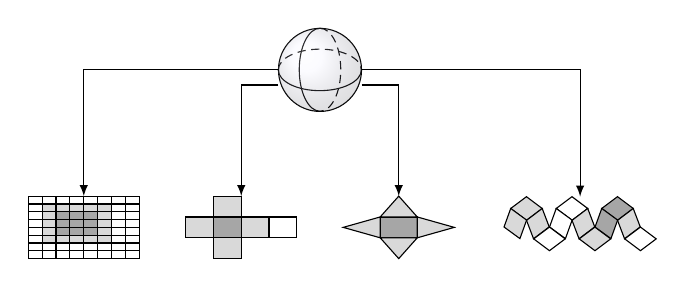
\begin{tikzpicture}
\tikzset{
	spherical/.pic={
		\draw (-0.0352778*#1,0) arc (180:360:#1 pt and 0.5*#1 pt);
	    \draw[densely dashed] (-0.0352778*#1,0) arc (180:0:#1 pt and 0.5*#1 pt);
   	    \draw (0,0.0352778*#1) arc (90:270:0.5*#1 pt and #1 pt);
   	    \draw[densely dashed] (0,0.0352778*#1) arc (90:-90:0.5*#1 pt and #1 pt);
     	\draw (0,0) circle (#1 pt);
     	\shade[ball color=blue!10!white,opacity=0.20] (0,0) circle (#1 pt);
    }
}

\tikzset{
	pics/equirectangular/.style n args={3}{
		code={
			%mid-quality
			\draw[fill=gray!30] (#2*0.00881945*#1-2*0.00881945*#1,#3*0.004961*#1-2*0.004961*#1) 
			rectangle 
			(#2*0.00881945*#1+3*0.00881945*#1,#3*0.004961*#1+3*0.004961*#1);

			%full-quality
			\draw[fill=gray!70] (#2*0.00881945*#1-0.00881945*#1,#3*0.004961*#1-0.004961*#1) 
			rectangle 
			(#2*0.00881945*#1+2*0.00881945*#1,#3*0.004961*#1+2*0.004961*#1);
			
			%grid
			\foreach \i in {-4,-3,-2,-1,0,1,2,3}{
				\foreach \j in {-4,-3,-2,-1,0,1,2,3}{
					\draw (\i*0.00881945*#1,\j*0.004961*#1) rectangle (\i*0.00881945*#1+0.00881945*#1,\j*0.004961*#1+0.004961*#1);
					}
				}
		}% code
	}% pic style
}%tikzset

\tikzset{
	cubemap/.pic={
		\draw[fill=gray!30] (-0.0352778*#1,-0.006615*#1) rectangle (-0.017639*#1,0.006615*#1);
		\draw[fill=gray!70] (-0.017639*#1,-0.006615*#1) rectangle (0,0.006615*#1);
		\draw[fill=gray!30] (0,-0.006615*#1) rectangle (0.017639*#1,0.006615*#1);
		\draw[fill=white] (0.017639*#1,-0.006615*#1) rectangle (0.0352778*#1,0.006615*#1);
		\draw[fill=gray!30] (-0.017639*#1,0.006615*#1) rectangle (0,0.019844*#1);
		\draw[fill=gray!30] (-0.017639*#1,-0.006615*#1) rectangle (0,-0.019844*#1);		
%		\draw[draw=black,fill=none] (-0.0352778*#1,-0.006615*#1) rectangle (0.0352778*#1,0.006615*#1);
	}
}

\tikzset{
	pyramid/.pic={
		\draw[fill=gray!70] (-0.011759*#1,-0.006615*#1) rectangle (0.011759*#1,0.006615*#1);
		% triangle north
		\draw[fill=gray!30] (-0.011759*#1,0.006615*#1)
			 -- (0.011759*#1,0.006615*#1)
			 -- (0,0.019844*#1)
			 -- cycle;
		% triangle south
		\draw[fill=gray!30] (-0.011759*#1,-0.006615*#1)
			 -- (0.011759*#1,-0.006615*#1)
			 -- (0,-0.019844*#1)
			 -- cycle;
		% triangle west
		\draw[fill=gray!30] (-0.011759*#1,-0.006615*#1)
			 -- (-0.011759*#1,0.006615*#1)
			 -- (-0.0352778*#1,0)
			 -- cycle;
		% triangle east
		\draw[fill=gray!30] (0.011759*#1,-0.006615*#1)
			 -- (0.011759*#1,0.006615*#1)
			 -- (0.0352778*#1,0)
			 -- cycle;
	}
}

\tikzset{
	pics/losange/.style n args={3}{
		code={
			\draw[fill=#2, rotate around={#3:(0,0)}] 
				(0,0) 
				-- (#1, 0.75*#1)
				-- (2*#1, 0)
				-- (#1, -0.75*#1)
				--	cycle;
		}
	}
}

\tikzset{
	dodecahedron/.pic={		
		\def\xshi{0}
		\pic at(\xshi,0) {losange={#1}{white}{0}};
		\pic at(\xshi,0) {losange={#1}{white}{287}};
		\pic at(\xshi+2*#1,0) {losange={#1}{gray!30}{254}};
		\pic at(\xshi+1.46*#1,-1.93*#1) {losange={#1}{gray!30}{0}};
		
		\def\xshi{2.89*#1}
		\pic at(\xshi,0) {losange={#1}{gray!70}{0}};
		\pic at(\xshi,0) {losange={#1}{gray!70}{287}};
		\pic at(\xshi+2*#1,0) {losange={#1}{gray!30}{254}};
		\pic at(\xshi+1.46*#1,-1.93*#1) {losange={#1}{white}{0}};	
		
		\def\xshi{-2.89*#1}%5.78
		\pic at(\xshi,0) {losange={#1}{gray!30}{0}};
		\pic at(\xshi,0) {losange={#1}{gray!30}{287}};
		\pic at(\xshi+2*#1,0) {losange={#1}{gray!30}{254}};
		\pic at(\xshi+1.46*#1,-1.93*#1) {losange={#1}{white}{0}};
	}
}

\def\sizeSphere{20}%pt
\def\ecartY{-2}%cm
\def\ecartX{6}

% da sphere
\pic [local bounding box=spher]  at (0,0) {spherical=15};

% recantagular
\pic [local bounding box=equi] at (-3,\ecartY) {equirectangular={\sizeSphere}{-1}{0}};

% cupe map
\pic [local bounding box=cubemap] at (-1,\ecartY) {cubemap=\sizeSphere};

% pyramid
\pic [local bounding box=pyra] at (1,\ecartY) {pyramid=\sizeSphere};

% rhombic
%\pgfdeclareimage[width=36 pt]{dodecahedron}{RhombicDodecahedron.png}
%\node at (3,\ecartY) (dodec)
%    {\pgfbox[center,center]{\pgfuseimage{dodecahedron}}};
    
\def\unitused{0.2}

\pic [local bounding box=dodeca] at (3,0.88*\ecartY) {dodecahedron=\unitused};

% links
\draw[-latex] (spher.180) -| (equi);
\draw[-latex] (spher.200) -| (cubemap);
\draw[-latex] (spher.340) -| (pyra);
\draw[-latex] (spher) -| (dodeca);





\end{tikzpicture}
\caption{Mappings}
\end{figure}

\subsubsection{Equirectangular}

\subsubsection{Cube Maps}

\subsubsection{Pyramid}

\subsubsection{Rhombic Dodecahedron}

\section{Quality-Differentiated Mapping Evaluation}

\subsection{Evaluation Platform}

\subsection{Results}

\section{Discussion and Conclusion}

\newpage
%%%%%%%%%%%%%%%%%%%%%%%%%%%%%%%
%\bibliographystyle{IEEEtran}
%\bibliographystyle{IEEEbib}
\bibliographystyle{abbrvnat}  
%\bibliographystyle{abbrv}  
\bibliography{biblio}

\end{document}

